\documentclass[fleqn, xcolor=x11names]{beamer}
\usetheme{Frankfurt} % шаблон
\usecolortheme{default} % цветовая схема
\usepackage[11pt]{moresize}
\usepackage{multimedia}
\usepackage[T1]{fontenc}
\usepackage{pgfplots}
\usepackage[utf8]{inputenc}
\usepackage[russian]{babel}
\usepackage{media9}
\usepackage{listings}
\usepackage{amsmath}
\usepackage{color}
\usepackage{parskip}
\usepackage{wrapfig}
\usepackage{algorithmicx}
\usepackage{algorithm}
\usepackage{upgreek}
\usepackage{hyperref}


\usepackage{graphicx}
\lstdefinestyle{myLatexStyle}{
    basicstyle=\small\ttfamily,
    language={python},
    numbersep=5mm, numbers=left, numberstyle=\tiny, % number style
    breaklines=true,frame=single,framexleftmargin=8mm, xleftmargin=8mm,
    backgroundcolor=\color{green!5}, frameround=fttt,escapeinside=??,
    rulecolor=\color{red},
    morekeywords={% Give keywords here
        numpy},
    keywordstyle=\color[rgb]{0,0,1},                    % keywords
        commentstyle=\color[rgb]{0.133,0.545,0.133},    % comments
        stringstyle=\color[rgb]{0.627,0.126,0.941}  % strings
}
\lstset{style=myLatexStyle}

\setbeamertemplate{navigation symbols}{}
\setbeamertemplate{footline}{%
    \hspace{0.9\paperwidth}%
    \usebeamerfont{title in head/foot}%
    \insertframenumber\,/\,\inserttotalframenumber%
}



\title{Inductive Representation Learning on Temporal Graphs}
\author[Медведев~Д.\,В.]{Медведев Алексей Владимирович}
\institute[ВМК МГУ]{МГУ имени М. В. Ломоносова,
факультет ВМК, кафедра ММП}
\date{} 

\begin{document}

\begin{frame}
\maketitle
\end{frame}

\begin{frame}\frametitle{GNNs}

\begin{figure}[h]
\begin{center}
\includegraphics[scale=0.18]{/home/alex/python/Master_course/scientific_diary_2019-2020/slides/pics/GCNN-major.png}
\end{center}
\end{figure}

\begin{block}{Architecture}
\begin{itemize}

\item \textbf{Spectral}: based on graph Laplacian. Solves only \textbf{transductive} tasks.

\item \textbf{Spatial}: based on neighborhood aggregation via spatial operator. Solves both \textbf{inductive} and \textbf{transductive tasks}.
\end{itemize}
\end{block}
\end{frame}


\begin{frame}\frametitle{Task types}

\begin{table}[h!]
\begin{center}
\begin{tabular}{cc}
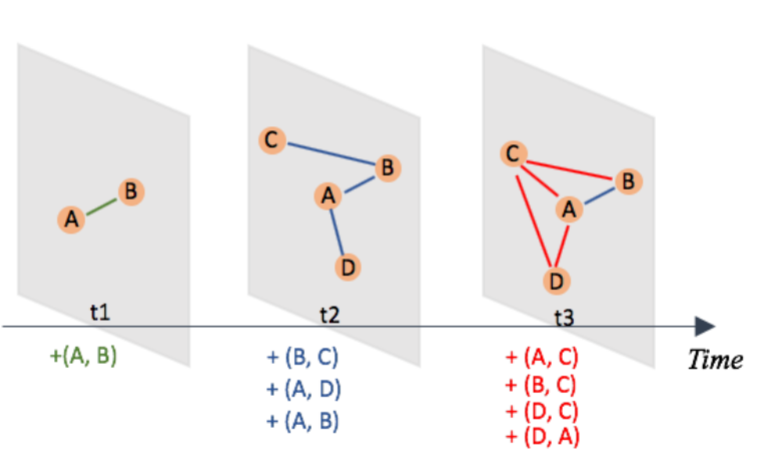
\includegraphics[scale=0.2]{/home/alex/python/Master_course/scientific_diary_20_21/slides/temporal_gcns/pics/time_snapshots.png} &
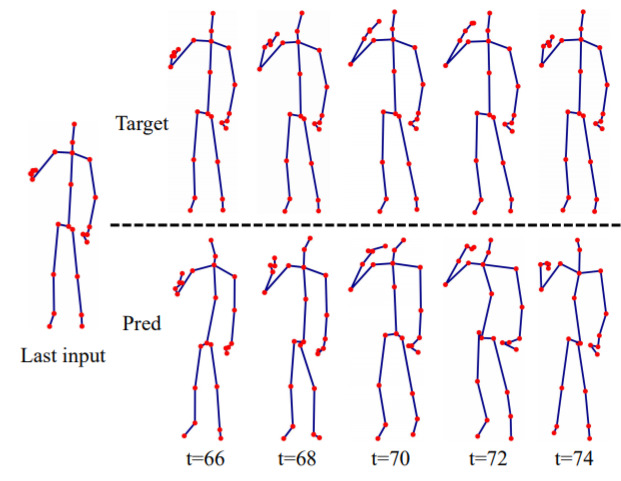
\includegraphics[scale=0.2]{/home/alex/python/Master_course/scientific_diary_20_21/slides/temporal_gcns/pics/Skeleton.png}\\
Inductive & Transductive\\
\end{tabular}
\end{center}
\end{table}

\end{frame}

\begin{frame}\frametitle{Continuous-Time Dynamic Network Embeddings\\ (Nguyen et al., 2018)}

\begin{figure}[h]
\begin{center}
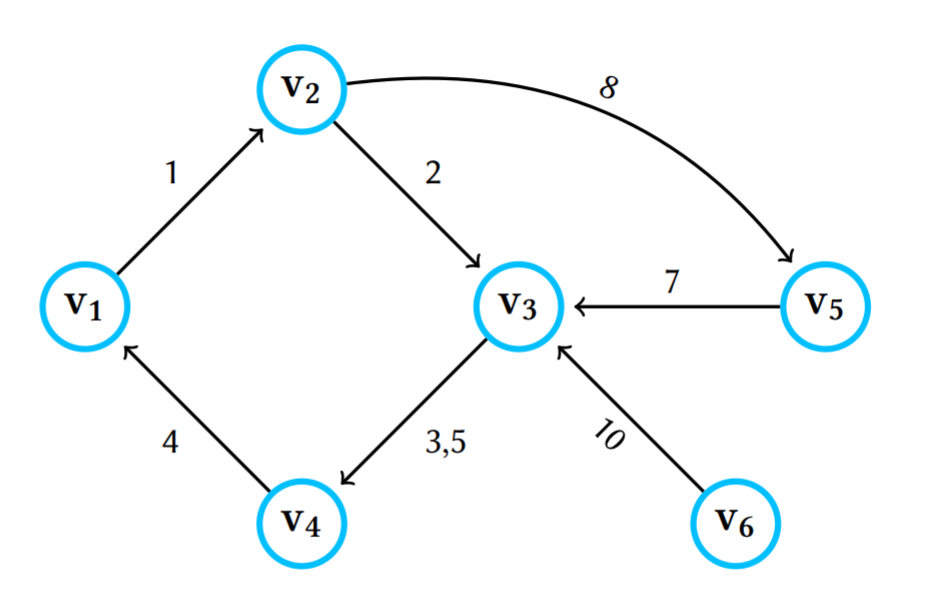
\includegraphics[scale=0.18]{/home/alex/python/Master_course/scientific_diary_20_21/slides/temporal_gcns/pics/time_graph.png}
\end{center}
\end{figure}

\begin{block}{Continuous-Time Dynamic Network}
$G = (V, E_T , \mathcal{T})$ , $V$ is a set of vertices, and $E_T \subseteq V \times V \times \mathbb{R}^{+}$
is the set of temporal edges, and $T : E \rightarrow \mathbb{R}^{+}$
is a function that maps each edge to a corresponding timestamp.
\end{block}


\end{frame}

\begin{frame}\frametitle{Continuous-Time Dynamic Network Embeddings}

\begin{figure}[h]
\begin{center}
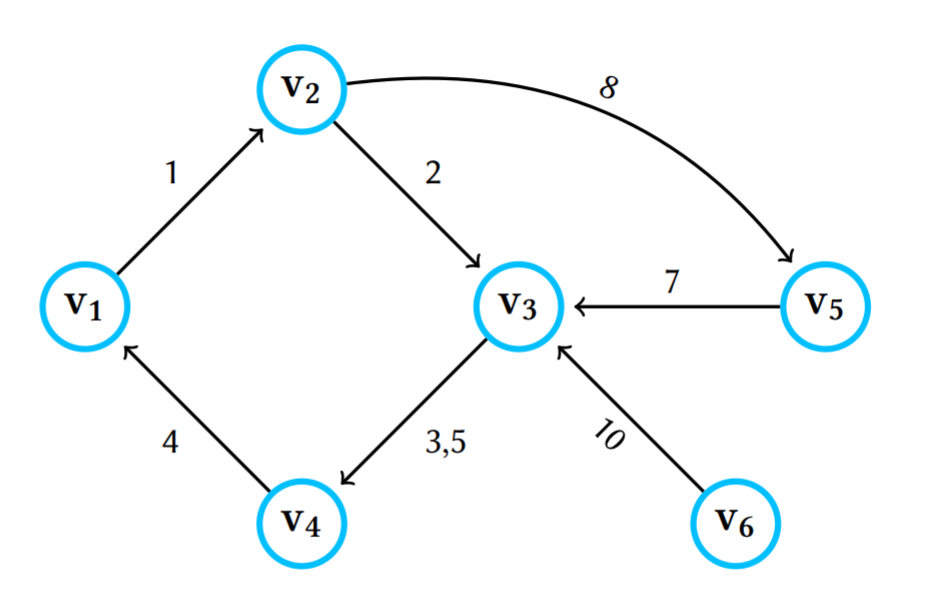
\includegraphics[scale=0.18]{/home/alex/python/Master_course/scientific_diary_20_21/slides/temporal_gcns/pics/time_graph.png}
\end{center}
\end{figure}

\begin{block}{Temporal Walk}
$\langle v_1,v_2, \dots ,v_k\rangle$ such that 
$\langle v_i, v_{i+1}\rangle \in E_T, \, 1 \le i < k$, and 
$\mathcal{T}(v_i,v_{i+1}) \le \mathcal{T}(v_{i+1},v_{i+2}),\, 1 \le i < (k-1)$.
\end{block}
\end{frame}

\begin{frame}\frametitle{Continuous-Time Dynamic Network Embeddings}

\begin{figure}[h]
\begin{center}
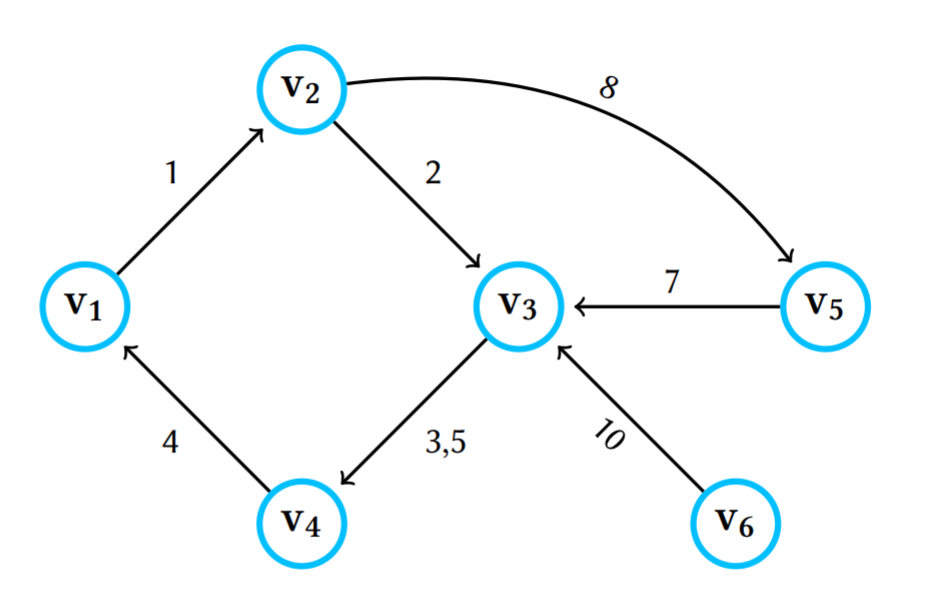
\includegraphics[scale=0.18]{/home/alex/python/Master_course/scientific_diary_20_21/slides/temporal_gcns/pics/time_graph.png}
\end{center}
\end{figure}

\begin{block}{Temporal Neighborhood}
$ \Gamma_t(v) = \left\lbrace (w, t') \mid e=(v,w,t') \in E_T \wedge \mathcal{T}(e) > t  \right\rbrace $
\end{block}

\begin{block}{Goal}
Given $G = (V, E_T , \mathcal{T})$ goal is to learn 
$f:\: V \rightarrow \mathbb{R}^D$, that maps nodes to representations suitable for a down-stream machine learning
task such as temporal link prediction.
\end{block}

\end{frame}

\begin{frame}\frametitle{Continuous-Time Dynamic Network Embeddings}

\begin{block}{Initial Temporal Edge Selection}

\textbf{Unbiased}:
$$ \text{Pr}(e) = 1/|E_T| $$
\textbf{Exponential}:
$$ \text{Pr}(e) = \frac{\exp\left[\mathcal{T}(e)-t_{\text{min}} \right]}{\sum \limits_{e' \in E_T} 
\exp\left[\mathcal{T}(e')-t_{\text{min}} \right]} $$
\textbf{Linear}:
$$ \text{Pr}(e) = \frac{\text{rank-asc}(e)}{\sum \limits_{e' \in E_T} \text{rank-asc}(e')} $$
\end{block}

\end{frame}

\begin{frame}\frametitle{Continuous-Time Dynamic Network Embeddings}

\begin{block}{Temporal Random Walk}

\textbf{Unbiased}:
$$ \text{Pr}(w) = 1/|\Gamma_t(v)| $$
\textbf{Exponential}:
$$ \text{Pr}(w) = \frac{\exp\left[\tau(w)-\tau(v) \right]}{\sum \limits_{w' \in \Gamma_t(v)} 
\exp\left[\tau(w')-\tau(v) \right]} $$
\textbf{Linear}:
$$ \text{Pr}(w) = \frac{\text{rank-desc}(w)}{\sum \limits_{w' \in \Gamma_t(v)} \text{rank-desc}(w')} $$
\end{block}

\end{frame}

\begin{frame}\frametitle{Continuous-Time Dynamic Network Embeddings}

\begin{block}{Optimization problem}
$$ \max \limits_f \log \text{Pr} \left(
W_T = \left\lbrace v_{i-w}, \dots , v_{i+w} \right\rbrace 
\setminus v_i \mid f(v_i) \right),$$
$$  \mathcal{T} (v_{i-\omega},v_{i-\omega+1}) < \dots < \mathcal{T} (v_{i+\omega-1},v_{i+\omega})$$
$$ \text{Pr} \left(W_T \mid f(v_i) \right)
= \prod \limits_{v_{i+k} \in W_T} \text{Pr} \left(v_{i+k} \mid f(v_i) \right) = 
 $$
 $$\text{Pr} \left(n \mid f(u) \right)  =  \frac{\exp(f(n)f(u))}{\sum \limits_{v \in V} \exp(f(v)f(u))},\, O(V) $$
 

\end{block}

\end{frame}

\begin{frame}\frametitle{Continuous-Time Dynamic Network Embeddings}

\begin{figure}[h]
\begin{center}
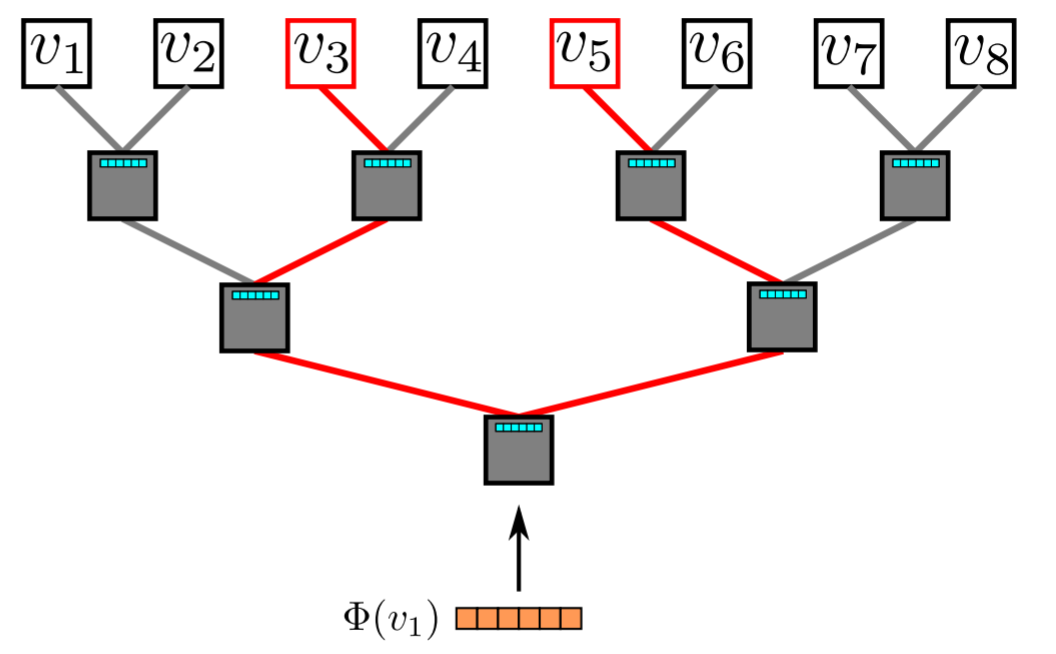
\includegraphics[scale=0.18]{/home/alex/python/Master_course/scientific_diary_20_21/slides/temporal_gcns/pics/HierarchicalSoftmax.png}
\end{center}
\end{figure}

\begin{block}{Hierarchical Softmax}
$$ \text{Pr} \left(n \mid f(u) \right)  =  \prod \limits_{l=1}^{\log |V|} \text{Pr}(b_l \mid f(u)),\, O(\log|V|) $$
\end{block}

\end{frame}

\begin{frame}\frametitle{Continuous-Time Dynamic Network Embeddings}
\begin{figure}[h]
\begin{center}
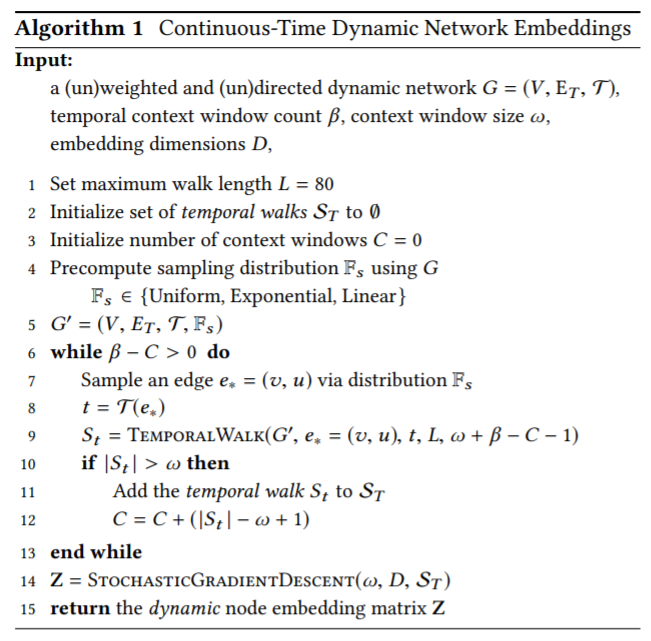
\includegraphics[scale=0.35]{/home/alex/python/Master_course/scientific_diary_20_21/slides/temporal_gcns/pics/CTDNE_alg.png}
\end{center}
\end{figure}
\end{frame}

\begin{frame}\frametitle{Inductive Representation Learning on Temporal Graphs\\
(Xu et al., 2020)}


\begin{figure}[h]
\begin{center}
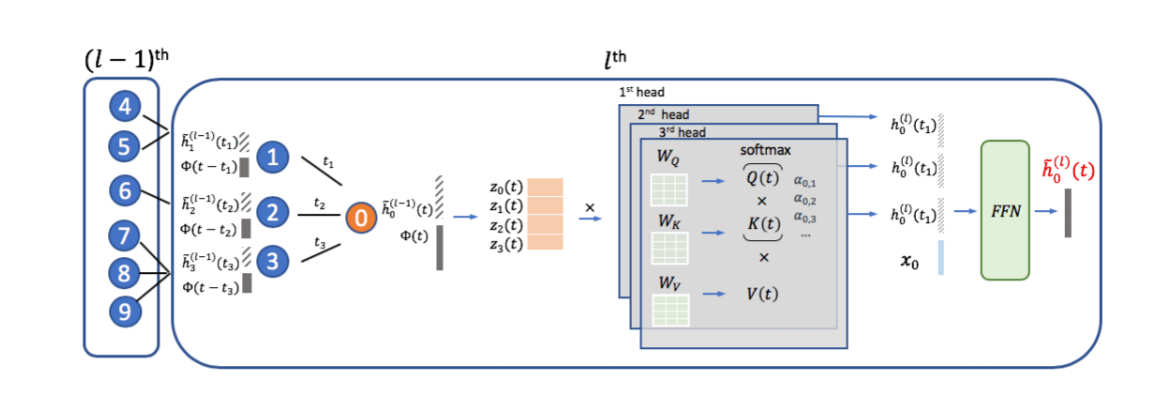
\includegraphics[scale=0.25]{/media/alex/Data/python/Master_course/scientific_diary_20_21/pics/TGAT_architecture.png}
\end{center}
\end{figure}

\begin{block}{Motivation}
Nguyen et al. (2018) approach only generates
embeddings for the \textbf{final} state of temporal graph and \textbf{transductive}.
\end{block}

\end{frame}

\begin{frame}\frametitle{Inductive Representation Learning on Temporal Graphs}

\begin{block}{Self Attention}
$$ Z_e = \left[ z_{e_1} + p_1, \dots, z_{e_l} + p_l \right]^T \in \mathbb{R}^{l \times d}, \,$$
$$ Z_e = \left[ z_{e_1} || p_1, \dots, z_{e_l} || p_l \right]^T \in \mathbb{R}^{l \times d+d_l}$$
Where $z_{e_i}$ -- input embeddings and $p_i$ -- positional embeddings.
$$ \text{Attn}(Q, K, V) = \text{softmax}\left( \frac{QK^T}{\sqrt{d}}V \right)$$
$$Q = Z_e W_Q,\, K = Z_e W_k, V = Z_e W_V$$
\end{block}

\end{frame}

\begin{frame}\frametitle{Inductive Representation Learning on Temporal Graphs}

\begin{block}{Kernel Trick}
$$ F: T \rightarrow R^{d_T},\, K(t_1, t_2) = \langle F(t_1), F(t_2) \rangle = \psi(t1-t2) $$
\end{block}

\begin{block}{Bochner’s Theorem}

A continuous, translation-invariant kernel $K(t_1, t_2) =  \psi(t1-t2)$
is positive definite if and only if there exists a non-negative measure on $\mathbb{R}$ such that $\psi$ is the
Fourier transform of the measure.

\end{block}

$$ \psi(t1-t2) = \int \limits_{\mathbb{R}} \exp \left(iw(t_1 - t_2) \right) p(w) dw
 = \mathbb{E}_w \left[ \upxi_w(t_1) \upxi_w(t_2)^{*}  \right] = 
 $$ 
$$ = \mathbb{E}_w \left[ \cos(w(t_1-t_2)) \right] 
= \mathbb{E}_w \left[ \cos(wt_1)\cos(wt_2) + \sin(wt_1)\sin(wt_2)  \right] \approx $$
$$ \approx \frac{1}{d} \sum \limits_{i=1}^{d} 
\cos(w_it_1)\cos(w_it_2) + \sin(w_it_1)\sin(w_it_2); \, w_1, \dots, w_d \sim p(w)$$


\end{frame}

\begin{frame}\frametitle{Inductive Representation Learning on Temporal Graphs}

$$ F_d(t) = \sqrt{\frac{1}{d}} \left[\cos(w_1t),\sin(w_1t),\dots,   \cos(w_dt),\sin(w_dt) \right],$$

\begin{block}{Claim 1}
Let $p(w)$ be the corresponding probability measure stated in Bochner’s Theorem for kernel function $K$.  Suppose the feature map $F$  is constructed using samples $\left\lbrace w_i \right\rbrace_{i=1}^d$, then we only need $  d = \Omega \left( \frac{1}{\epsilon^2} \log \frac{\sigma^2_p t_{\max}}{\epsilon} \right) $ 
samples to have
$$ \sup \limits_{t_1, t_2 \in T} | F_d(t_1)^T F_d(t_2) - K(t_1, t_2)| < \epsilon$$ with any probability $\forall\epsilon > 0 $ where $ \sigma^2_p $ 
is the second momentum with respect to $p(w)$
\end{block}

\end{frame}

\begin{frame}\frametitle{Inductive Representation Learning on Temporal Graphs}

\begin{block}{Notation}
\begin{itemize}
\item $v_i$ is a vertex
\item $x_i$ is corresponding feature vector
\item $ \hat{h}_i^l(t) $ output for node $i$ at time $t$ from the $l$'th layer
\item $N(v_0; t) = \left\lbrace v_1, \dots, v_N \right\rbrace $ -- neighborhood for node $v_0$ at time $t$. $v_0, v_i \in N(v_0; t) \Leftrightarrow (v_0, v_i, t_i) \in G, t_i < t $
\end{itemize}
\end{block}

\begin{block}{temporal graph attention layer (TGAT layer)}

$$Z(t) = \left[\hat{h}_0^{l-1}(t)||F_{d_T}(0), \dots, \hat{h}_N^{l-1}(t_N)||F_{d_T}(t-t_N) \right]$$
$$ q(t) = \left[ Z(t) \right]_0W_Q, 
K(t) = \left[ Z(t) \right]_{1:N}W_K, V(t) = \left[ Z(t) \right]_{1:N}W_V$$
$$ \alpha_i = \exp\left(q^TK_i \right)/\left( \sum \limits_q \exp \left( q^T K_q \right) \right) $$

$$ h(t) = \text{Attn}\left(q(t), K(t), V(t) \right) \in \mathbb{R}^{d_h} $$

\end{block}

\end{frame}

\begin{frame}\frametitle{Inductive Representation Learning on Temporal Graphs}

\begin{figure}[h]
\begin{center}
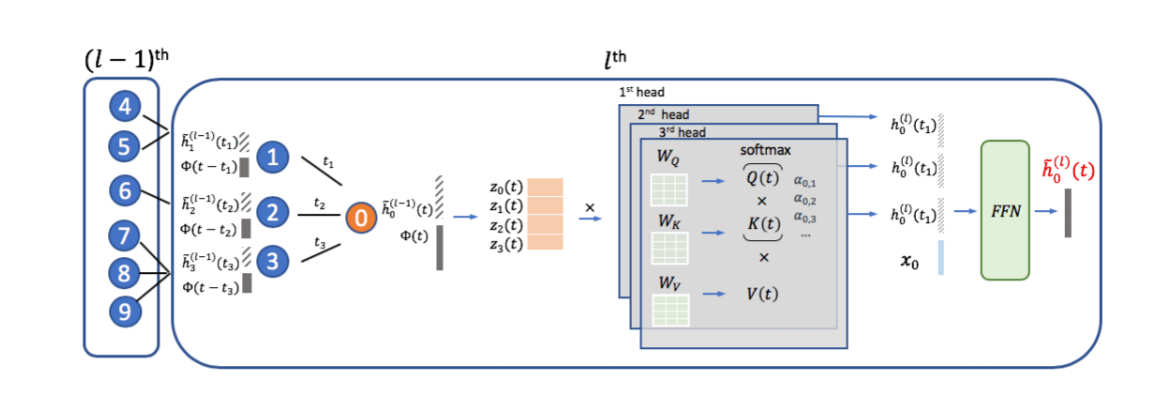
\includegraphics[scale=0.25]{/media/alex/Data/python/Master_course/scientific_diary_20_21/pics/TGAT_architecture.png}
\end{center}
\end{figure}

\begin{block}{temporal graph attention layer (TGAT layer)}
$$ \hat{h}_0^l(t) = \text{FFN}\left( h(t)||x_0 \right)
= \text{ReLU} \left( \left[ h(t)||x_0 \right] W^l_0 + b_0^l \right)W_1^l + b_1^l, $$
$$ W_0^l \in \mathbb{R}^{(d_h + d_0) \times d_f}, W_1^l \in \mathbb{R}^{d_f \times d}, b_0^l \in \mathbb{R}^{d_f}, b_1^l \in \mathbb{R}^d  $$
\end{block}

\end{frame}

\begin{frame}\frametitle{Inductive Representation Learning on Temporal Graphs}

\begin{figure}[h]
\begin{center}
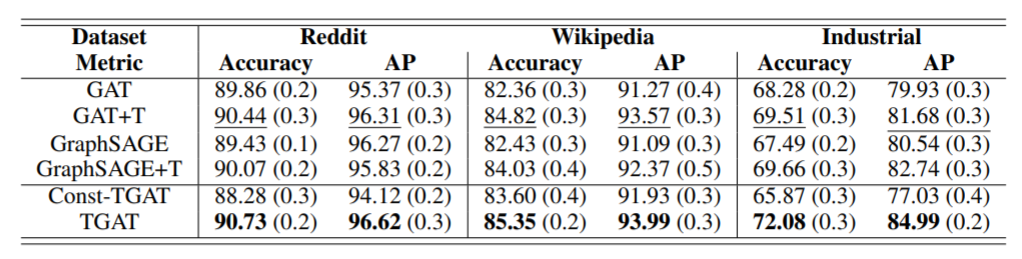
\includegraphics[scale=0.25]{/media/alex/Data/python/Master_course/scientific_diary_20_21/pics/Results.png}
\end{center}
\end{figure}

\begin{figure}[h]
\begin{center}
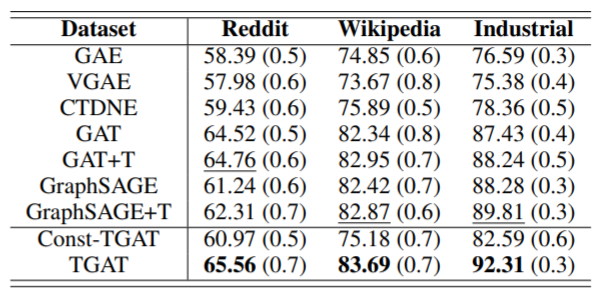
\includegraphics[scale=0.25]{/media/alex/Data/python/Master_course/scientific_diary_20_21/pics/Downstream.png}
\end{center}
\end{figure}

\end{frame}

\begin{frame}\frametitle{References}

\begin{itemize}
\item Da Xu, Chuanwei Ruan, Evren Korpeoglu, Sushant Kumar, Kannan Achan.\\
\href{https://openreview.net/pdf?id=rJeW1yHYwH}{Inductive Representation Learning on Temporal Graphs}\\
International Conference on Learning Representations (ICLR), 2020.

\item Giang Hoang Nguyen, John Boaz Lee, Ryan A Rossi, Nesreen K Ahmed, Eunyee Koh, and Sungchul Kim.\\
Continuous-time dynamic network embeddings.\\
In Companion Proceedings of
the The Web Conference 2018, pp. 969–976. International World Wide Web Conferences Steering
Committee, 2018.

\item Bryan Perozzi, Rami Al-Rfou, and Steven Skiena.\\
Deepwalk: Online learning of social representations.\\
pp. 701–710. ACM, 2014.

\end{itemize}

\end{frame}

\begin{frame}\frametitle{References}
\begin{itemize}
\item Aditya Grover and Jure Leskovec.\\
node2vec: Scalable feature learning for networks.\\
pp. 855–864. ACM, 2016.

\item Petar Velickovic, Guillem Cucurull, Arantxa Casanova, Adriana Romero, Pietro Lio, and Yoshua Bengio.\\
Graph attention networks.\\
arXiv preprint arXiv:1710.10903, 2017.

\item Will Hamilton, Zhitao Ying, and Jure Leskovec.\\
Inductive representation learning on large graphs.\\
Advances in Neural Information Processing Systems,
pp. 1024–1034, 2017.


\end{itemize}
\end{frame}

\begin{frame}\frametitle{References}
\begin{itemize}
\item Da Xu, Chuanwei Ruan, Evren Korpeoglu, Sushant Kumar, and Kannan Achan.\\
Self-attention with functional time representation learning.\\
Advances in Neural Information Processing Systems,
pp. 15889–15899, 2019
\end{itemize}
\end{frame}

\end{document}

